\section{Gario}
\section{Gario}


\begin{figure}
\centering
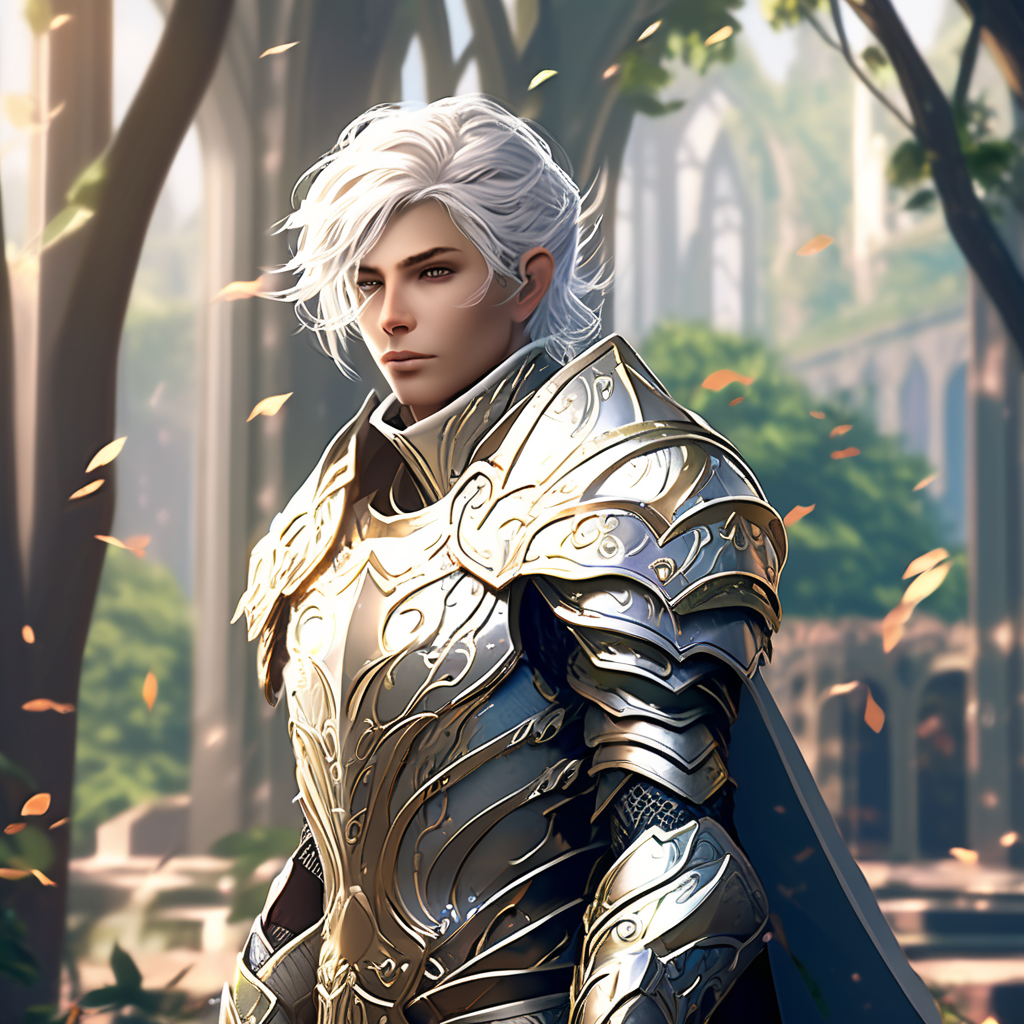
\includegraphics{depict-an-elf-paladin-he-is-a-young-adult-with-short-white-hairs-wearing-full-plate-armour.png}
\caption{depict-an-elf-paladin-he-is-a-young-adult-with-short-white-hairs-wearing-full-plate-armour.png}
\end{figure}

Informazioni Generali

Età: 623

Data di nascita:

Luogo di nascita: Fredo Flu

Razza: Elfo

Classe: Paladino

Alleati:

Nemesi: Le Zucche

Alias:

Professione:


\subsection{1. Descrizione Generale}\label{descrizione-generale}


\begin{figure}
\centering
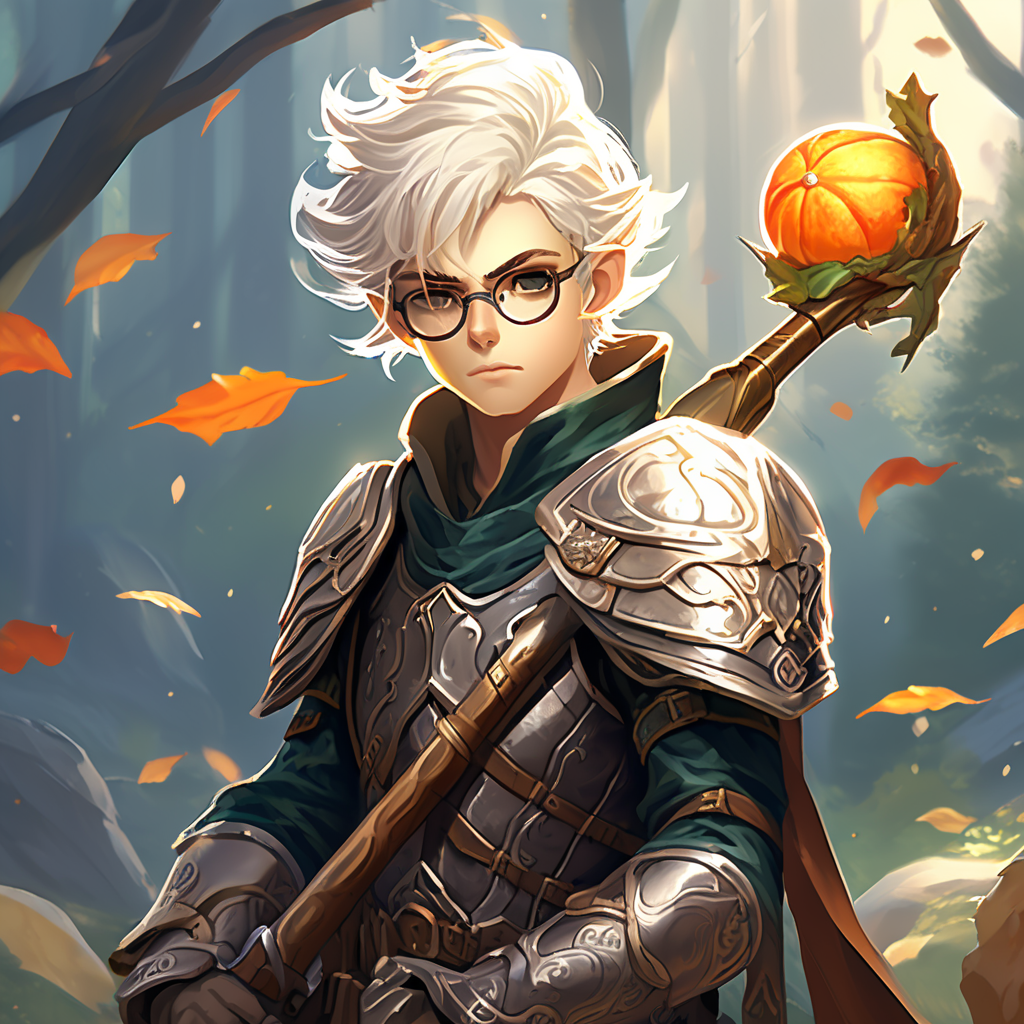
\includegraphics{depict-an-elf-paladin-he-is-a-young-adult-with-short-white-hairs-wearing-full-plate-armour-and-spe-923031639.png}
\caption{depict-an-elf-paladin-he-is-a-young-adult-with-short-white-hairs-wearing-full-plate-armour-and-spe-923031639.png}
\end{figure}

Gario è un elfo paladino di Fredo Flu, con una personalità complessa.
Sebbene animato da un senso di giustizia, è bigotto, xenofobo e
ipocrita, credendo di agire per il bene supremo. Dietro la durezza, ha
un cuore compassionevole, ma le sue azioni spesso suscitano polemiche.

\begin{quote}
``Io le feste di autunno non le voglio festeggiare'' - Gario Miordano
\end{quote}

\subsection{2. Biografia}\label{biografia}


\subsubsection{\texorpdfstring{\textbf{2.1 Origini Nobili e Caduta di
Fredo
Flu}}{2.1 Origini Nobili e Caduta di Fredo Flu}}\label{origini-nobili-e-caduta-di-fredo-flu}

Gario Miordano è nato all'interno di una delle più illustri famiglie
elfiche di Fredo Flu, un tempo una delle città più fiorenti e prosperose
del regno elfico. Cresciuto tra l'agio e il lusso, Gario ha goduto di
una vita privilegiata fin dalla sua infanzia, circondato dall'amore e
